\documentclass[tikz,border=6pt]{standalone}
\usepackage{pgfplots}
\pgfplotsset{compat=1.18}
\usepgfplotslibrary{colormaps}
\usetikzlibrary{arrows, arrows.meta, calc}
\usetikzlibrary{decorations.markings}


\usepackage{amssymb,amsmath,mathtools}

\usepackage[T1]{fontenc}
\usepackage[utf8]{inputenc}
\usepackage{newpxtext,newpxmath}
\usepackage{sectsty}

\renewcommand{\Re}{\operatorname{\mathrm{Re}}}
\renewcommand{\Im}{\operatorname{\mathrm{Im}}}

\begin{document}
	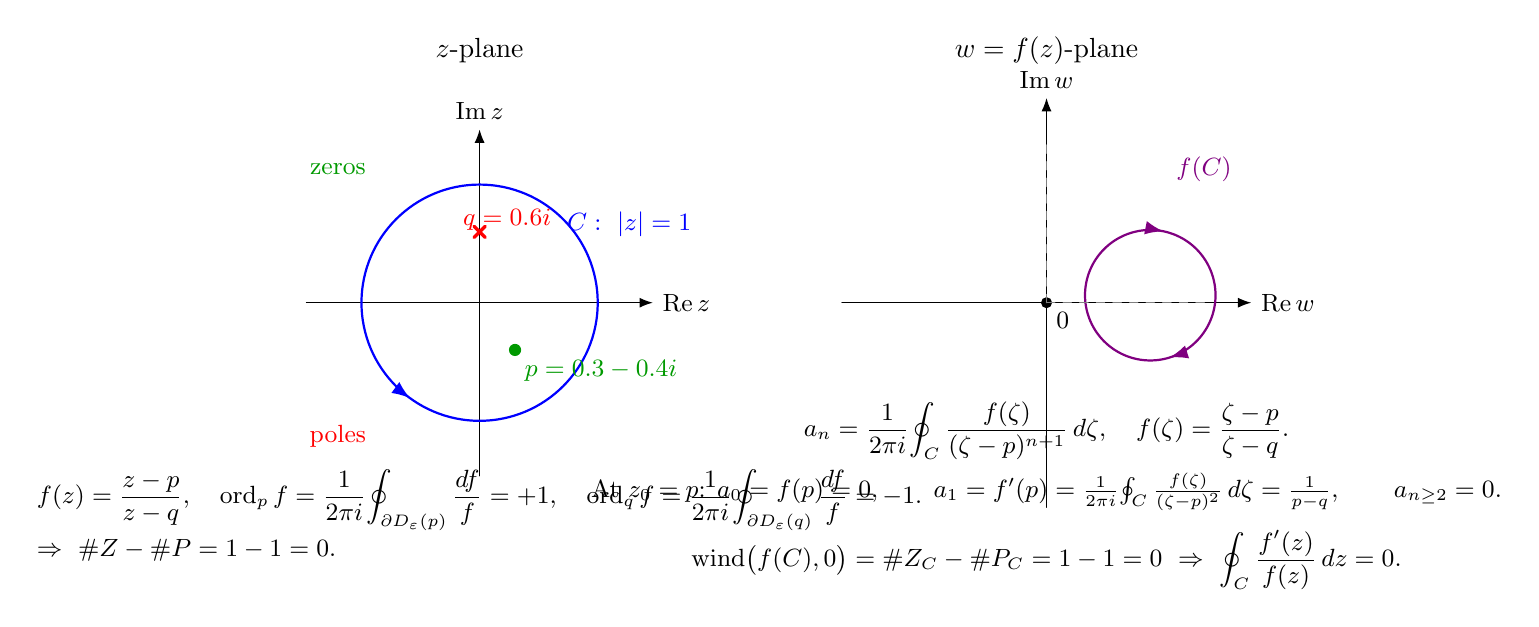
\begin{tikzpicture}[>=Latex, line cap=round, line join=round, font=\small]
		
		%========================
		% Left: z-plane
		%========================
		\begin{scope}[shift={(0,0)}]
			\node[font=\normalsize] at (0,3.2) {$z$-plane};
			% axes
			\draw[->] (-2.2,0)--(2.2,0) node[right] {$\Re z$};
			\draw[->] (0,-2.2)--(0,2.2) node[above] {$\Im z$};
			
			% unit circle C (positively oriented) -- drawn with radius 1.5 for visibility
			\draw[blue,thick,postaction={decorate},
			decoration={markings, mark=at position 0.65 with {\arrow{>}}}]
			(0,0) circle (1.5);
			\node[blue] at (1.9,1.0) {$C:\ |z|=1$};
			
			% zero at p (order +1) and pole at q (order -1)
			\fill[green!60!black] (0.45,-0.6) circle(2.2pt) node[below right] {$p=0.3-0.4i$};
			\node[green!60!black] at (-1.8,1.7) {zeros};
			\draw[red,very thick] (0,0.9) ++(-0.07,-0.07) -- ++(0.14,0.14);
			\draw[red,very thick] (0,0.9) ++(-0.07,0.07)  -- ++(0.14,-0.14);
			\node[red] at (0.35,1.05) {$q=0.6i$};
			\node[red] at (-1.8,-1.7) {poles};
			
			% function label + orders via winding/logarithmic derivative
			\node[align=left] at (0,-2.7) {$\displaystyle
				f(z)=\frac{z-p}{z-q},\quad
				\operatorname{ord}_{p} f
				=\frac{1}{2\pi i}\!\oint_{\partial D_\varepsilon(p)}\frac{df}{f}=+1,\quad
				\operatorname{ord}_{q} f
				=\frac{1}{2\pi i}\!\oint_{\partial D_\varepsilon(q)}\frac{df}{f}=-1.$\\[2pt]
				$\Rightarrow\ \#Z-\#P=1-1=0.$};
		\end{scope}
		
		%========================
		% Right: w-plane = f(z)-plane
		%========================
		\begin{scope}[shift={(7.2,0)}]
			\node[font=\normalsize] at (0,3.2) {$w=f(z)$-plane};
			% axes
			\draw[->] (-2.6,0)--(2.6,0) node[right] {$\Re w$};
			\draw[->] (0,-2.6)--(0,2.6) node[above] {$\Im w$};
			
			% origin
			\fill (0,0) circle(2pt) node[below right] {$0$};
			
			% image curve f(C): z = 1.5 e^{it} -> w = (z-p)/(z-q)
			% Let x = 1.5 cos t, y = 1.5 sin t.
			% N = (x-0.3) + i(y+0.4),  D = x + i(y-0.6).
			% Re w = (Nre*Dre + Nim*Dim)/|D|^2,  Im w = (Nim*Dre - Nre*Dim)/|D|^2.
			\draw[violet,thick,
			postaction={decorate},
			decoration={markings,
				mark=at position 0.20 with {\arrow{>}},
				mark=at position 0.62 with {\arrow{>}}}]
			plot[domain=0:6.283, samples=650]
			({
				( (1.5*cos(\x r)-0.3)* (1.5*cos(\x r))
				+ (1.5*sin(\x r)+0.4)* (1.5*sin(\x r)-0.6) )
				/
				( (1.5*cos(\x r))*(1.5*cos(\x r))
				+ (1.5*sin(\x r)-0.6)*(1.5*sin(\x r)-0.6) )
			},
			{
				( (1.5*sin(\x r)+0.4)* (1.5*cos(\x r))
				- (1.5*cos(\x r)-0.3)* (1.5*sin(\x r)-0.6) )
				/
				( (1.5*cos(\x r))*(1.5*cos(\x r))
				+ (1.5*sin(\x r)-0.6)*(1.5*sin(\x r)-0.6) )
			});
			\node[violet] at (2.0,1.7) {$f(C)$};
			
			% dashed rays to visualize winding
			\draw[gray,dashed] (0,0) -- (2.1,0);
			\draw[gray,dashed] (0,0) -- (0,2.1);
			
			% annotation: Taylor coefficients at z_0=p via Cauchy integrals
			\node[align=center] at (0,-2.45)
			{$\displaystyle
				a_n=\frac{1}{2\pi i}\!\oint_C \frac{f(\zeta)}{(\zeta-p)^{n+1}}\,d\zeta,\quad
				f(\zeta)=\frac{\zeta-p}{\zeta-q}.$\\[4pt]
				At $z_0=p$: $a_0=f(p)=0,\qquad
				a_1=f'(p)=\frac{1}{2\pi i}\!\oint_C \frac{f(\zeta)}{(\zeta-p)^{2}}\,d\zeta=\frac{1}{p-q},\qquad
				a_{n\ge2}=0.$\\[6pt]
				$\mathrm{wind}\big(f(C),0\big)=\#Z_C-\#P_C=1-1=0
				\ \Rightarrow\
				\displaystyle \oint_C \frac{f'(z)}{f(z)}\,dz=0.$};
		\end{scope}
		
	\end{tikzpicture}
\end{document}